\chapter{Introduzione}

Negli ultimi anni l'economia non è più incentrata sui beni, ma è incentrata sui servizi.\
È nata una tendenza a vedere ``tutto come un servizio'':\ bike sharing, car sharing, streaming musicale, cloud storage,\ \dots

La \textbf{Quality of Service} (QoS) è fondamentale per qualsiasi servizio che utilizziamo, non basta che sia conveniente economicamente ma deve anche essere affidabile.\
Le informazioni sull'affidabilità vengono scritte nel contratto che i clienti spesso (quasi sempre) ignorano e accettano senza leggere.

I clienti non sanno (e spesso non vogliono sapere) come è implementato il servizio che usano, scelgono (o dovrebbero scegliere) se usarlo o meno sulla base del contratto che è (o dovrebbe essere) esposto da chi fornisce il servizio.\
I termini di un contratto vengono definiti nel \textbf{Service Level Agreement} che è formulato da esperti.\
Un esempio di Service Level Agreement può essere quello di Facebook:

\vspace{12pt}
\noindent``\dots\textit{quando l'utente condivide, pubblica o carica un contenuto protetto da diritti di proprietà intellettuale in relazione o in connessione con i Prodotti di Facebook, concede una licenza non esclusiva, trasferibile, sub-licenziabile, non soggetta a royalty e valida in tutto il mondo per la trasmissione, l'uso, la distribuzione, la modifica, l'esecuzione, la copia, la pubblica esecuzione o la visualizzazione, la traduzione e la creazione di opere derivate dei propri contenuti}\dots''

\begin{center}
    Perché sono così importanti i dati che vengono messi sui Social Network?\
\end{center}
Nei colloqui di assunzione, alcuni specialisti di risorse umane cercano di valutare com'è una persona inizialmente dai Social Network.\
Una volta si facevano delle domande per capire il tipo di persona che avevamo davanti, ma oggi è tutto trasparente sui Social.\

\section{Cloud Computing}
La richiesta di un servizio può variare nel tempo, \textbf{nessuno} sa come.\
Quindi solitamente ci troviamo davanti due grandi problemi:
\begin{itemize}
    \item \textbf{Overprovisioning}:\ cercare di assicurarsi di soddisfare i picchi attesi di richieste (dovuti a pattern giornalieri, stagionali o picchi inattesi) porta a sprecare risorse (se la stima è corretta – ancora peggio se la richiesta è sovrastimata).
    \item \textbf{Underprovisioning}:\ se la richiesta è sottostimata allora underprovisioning può accidentalmente \textbf{respingere utenti}.\ Costo di underprovisioning più difficile da misurare, ma serio come quello di overprovisioning; non solo gli \textbf{utenti respinti} non generano entrate, \textbf{potrebbero non tornare mai più}.
\end{itemize}
Questi problemi erano molto più frequenti finché le risorse non erano virtualizzate, ma tutto è cambiato quando si è evoluto il Cloud.\
Il Cloud Computing offre una quantità di risorse, apparentemente infinite, e disponibili su richiesta.\
Il NIST (National Institute of Standards and Technology) l'ha definito come:

\vspace{12pt}
\noindent``\textit{Un modello per permettere un accesso via rete diffuso, conveniente e su richiesta a un insieme condiviso di risorse di calcolo configurabili}.\
\textit{Queste risorse possono essere rapidamente fornite e rilasciate con un minimo costo di gestione o di interazione col fornitore del servizio}.''

\subsubsection{Idee chiave}
\noindent Le idee chiave del Cloud Computing:
\begin{itemize} %riguardare
    \item raggruppare in modo efficiente e on-demand infrastrutture virtuali, offerte come servizi;
    \item fornire risorse dinamicamente scalabili, virtualizzate a molti clienti attraverso Internet;
    \item separare la fornitura dei servizi di calcolo dalla tecnologia sottostante (gli utenti non vedono l'infrastruttura).
\end{itemize}

\subsubsection{Attrattiva economica}
Il Cloud Computing attrae gli utenti per due motivi principali
\begin{itemize}
    \item Eliminazione di impegni ``in anticipo'' da parte degli utenti (elimina le spese di capitale CapEx e vengono convertite in spese di operazione OpEx).
    \item \textbf{Pay-per-use}:\ i clienti lo amano e anche se è più costoso, il costo è compensato dai benefici economici in termini di \textbf{elasticità} e \textbf{trasferimento dei rischi}.\ Il rischio è spostato sul Service Level Agreement.
\end{itemize}

\subsubsection{Modelli di Servizio}
Esistono vari modelli di servizio.

\textbf{ToP} (Tradition on Premise):\ faccio tutto ``in casa'' e non prendo servizi esterni.\

\textbf{SaaS} (Software as a Service) fornisce software on-demand accessibile mediante client thin o API.\
Il fornitore SaaS gestisce infrastruttura, sistema operativo e applicazione, mentre il cliente non è responsabile di niente.

\textbf{PaaS} (Platform as a Service) fornisce un'intera piattaforma come un servizio (machine virtuali, sistema operativo, servizi, ambiente di sviluppo).\
Il fornitore PaaS gestisce infrastruttura, sistema operativo e enabling software, mentre il cliente è responsabile di installare e gestire l'applicazione.\

\textbf{IaaS} (Internet as a Service) fornisce server, memoria, rete (virtualizzati).\
Il fornitore di servizi IaaS gestisce tutta l'infrastruttura, mentre il cliente è responsabile di tutti gli altri aspetti del deployment (p.e.\ sistema operativo, applicazione).

\begin{figure}[H]
    \centering
    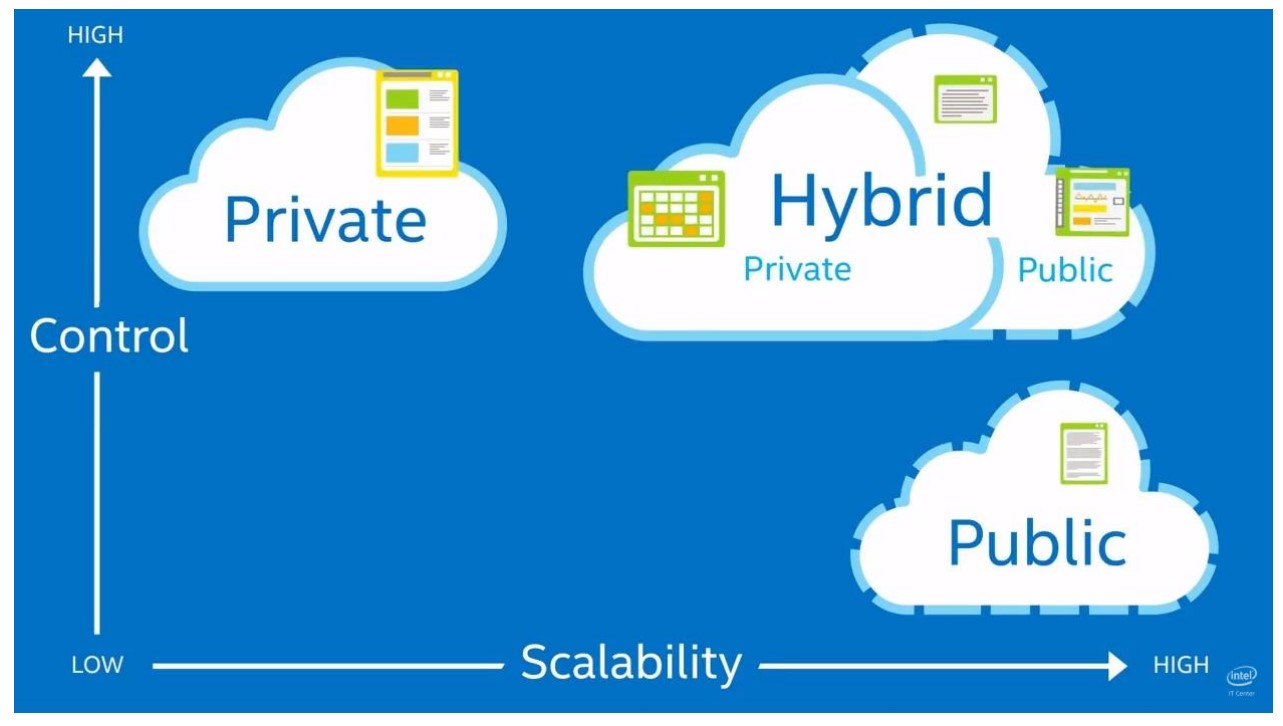
\includegraphics[width=0.7\textwidth]{immagini/Model_Deployment.jpg}
    \caption*{Model Deployment}
\end{figure}

\noindent Esistono modelli di deployment privati e pubblici, ma oggi sta avendo molto successo il Cloud ibrido:\ i dati sensibili sono mantenuti in privato, per esempio dentro l'azienda, e dove è necessaria più elasticità utilizzo un cloud pubblico.

\subsubsection{Perché si chiama Cloud?}

Perché quando si disegnava lo schema client-server tutto ciò che stava fra i due veniva rappresentato come una nuvoletta per semplicità.

\subsubsection{Ostacoli al Cloud}

\textbf{Confidenzialità dei dati}:\ Dove verranno memorizzati i nostri dati, concretamente?\ Privacy e integrità dei dati saranno garantiti?\ Come?\ Come sapremo se si è verificato un problema?

\noindent\textbf{Disponibilità dei servizi}:\ Cosa succede se un cloud provider fallisce?\ Mantra dell'informatica:\ ``no single point of failure\dots''

\noindent\textbf{Vendor lock-in}:\ rimanere ``bloccati'' con un fornitore di un servizio, per esempio dover pagare una penale per il recesso del contratto.

\section{Nuovi Modelli di Business}
Sono state innovative le idee di Dropbox, Spotify, Google.\
Dropbox ha deciso di offrire memoria gratuita a tutti, Spotify musica gratuita a tutti pagando i diritti ogni volta che viene riprodotta una canzone, mentre Google un motore di ricerca gratuito finanziandosi grazie al \textbf{customized advertising}.

\section{Green Computing}

Per costruire un computer ci vogliono due tonnellate di materiale grezzo, l'ICT in generale produce più emissioni di CO\textsubscript{2} degli aerei.\
Tra i fattori che contribuiscono all'inquinamento ci sono l'obsolescenza programmata e l'\textbf{obsolescenza} \textbf{percepita}:\ il venditore cerca di spingere il cliente ad acquistare un nuovo prodotto che avrà nuove funzionalità anche se al cliente queste non servono, ma il venditore farà in modo di fargli sentire questa ``mancanza''.\
Quindi c'è un gran numero di rifiuti tecnologici.\

In Arizona ci sono più di quaranta Data Center perché l'elettricità costa pochissimo, chiaramente le temperature del luogo richiedono grossi sistemi di raffreddamento che saranno sicuramente economici ma per niente ecologici.

